\documentclass[fleqn]{beamer}

\usepackage[british]{babel}
\usepackage{graphicx,ru,url}
\usepackage{amsmath,amsfonts}
% Use Times for math font and text font.
\RequirePackage[T1]{fontenc}
%\RequirePackage{txfonts}
% bold math must be loaded after Times font
\usepackage{bm}
\usepackage{booktabs} % nice rules (thick lines) for tables
\usepackage{microtype} % improves typography for PDF
\usepackage{xcolor}
\usepackage{tikz}
\usepackage{verbatim}
\usetikzlibrary{arrows,shapes, decorations}
\usepackage{hyperref}
% \usefonttheme{serif}

\providecommand{\e}[1]{\ensuremath{\times 10^{#1}}}

% The title of the presentation:
%  - first a short version which is visible at the bottom of each slide;
%  - second the full title shown on the title slide;
\title[KLT Basis for Energy Expansion]{
  Applications of the Karhunen-Lo\`{e}ve Transform for Basis Generation in the 
Response Matrix Method}

% Optional: a subtitle to be displayed on the title slide
%\subtitle{Show where you're from}

% The author(s) of the presentation:
%  - again first a short version to be displayed at the bottom;
%  - next the full list of authors, which may include contact information;
\author[Richard Reed]{
  Richard Reed \\
  rlreed@k-state.edu \\
  Under the guidance of Prof. Jeremy Roberts}

% The institute:
%  - to start the name of the university as displayed on the top of each slide
%    this can be adjusted such that you can also create a Dutch version
%  - next the institute information as displayed on the title slide
\institute[Kansas State University]{
  Mechanical and Nuclear Engineering \\
  Kansas State University}

% Add a date and possibly the name of the event to the slides
%  - again first a short version to be shown at the bottom of each slide
%  - second the full date and event name for the title slide
\date[Master's Defense]{
  Master's Defense \\
  17th April 2015}

\begin{document}
  %\renewcommand*{\inserttotalframenumber}{\pageref{lastframe}}
  \newcommand{\beginbackup}{
    \newcounter{framenumbervorappendix}
    \setcounter{framenumbervorappendix}{\value{framenumber}}
  }
  \newcommand{\backupend}{
    \addtocounter{framenumbervorappendix}{-\value{framenumber}}
    \addtocounter{framenumber}{\value{framenumbervorappendix}} 
  }
  
  \AtBeginSection[]{
  \begin{frame}
  \vfill
  \centering
  \begin{beamercolorbox}[sep=8pt,center,shadow=true,rounded=true]{title}
    \usebeamerfont{title}\insertsectionhead\par%
  \end{beamercolorbox}
  \vfill
  \end{frame}
}
  
  \begin{frame}
    \titlepage
  \end{frame}
  
  \begin{frame}
    \frametitle{Outline}
    \begin{block}{Presentation Outline}
      \begin{itemize}
          \item Motivation
          \item Introduction and Background
% 	\begin{itemize}
% 	  \item Response Matrix Method
% 	  \item Energy Expansion
% 	\end{itemize}
    \item Overview of Basis Sets
    \begin{itemize}
        \item Discrete Legendre Polynomials
        \item Modified Discrete Legendre Polynomials
        \item Karhunen-Lo\`{e}ve Transform
    \end{itemize}

	\item Test Problems and Models
	\begin{itemize}
	  \item 10-Pin Test Problem
	  \item BWR Test Problem
      \item C5G7 Test Problem
	\end{itemize}
	\item Results and Discussion
      \end{itemize}
    \end{block}
  \end{frame}
  
  \section{Motivation}
  
  \begin{frame}
      \frametitle{Project Motivation}
      \begin{block}{The Multigroup Neutron Transport Equation}
      \begin{equation*}
    \begin{split}
    \hat{\Omega}\cdot \nabla \psi_g(\hat{\Omega},\vec{r}) 
    &+ \Sigma_{t, g}\psi_g(\hat{\Omega},\vec{r}) = \\
    &\frac{1}{4\pi}\left[\sum^G_{g\prime = 1}\Sigma_{s,g\prime\rightarrow 
        g}\phi_{g\prime}(\vec{r}) + \frac{\chi_g}{k}\sum^G_{g\prime = 
        1}\nu\Sigma_{f,g\prime}\phi_{g\prime}(\vec{r})\right]
    \label{eq:multigroup}
\end{split}
\end{equation*}
\end{block}
\begin{block}{Challenges}
    \begin{itemize}
        \item 6(+1) Dimensions
        \item Group to Group Scattering
        \item Energy Dependence
    \end{itemize}

\end{block}

  \end{frame}
  
  \begin{frame}
      \frametitle{Project Motivation}
      \begin{block}{Attempt to model a PWR in 3-D} 
          \begin{itemize}
              \item 193 assemblies
              \item Each assembly is 17$\times$17 fuel pins
              \item 50 spatial cells radially per pincell
              \item 300 axial mesh points
              \item 100 energy groups
              \item 100 points in each angle
              \item Over 1\e{13} unknowns for only reactor core
          \end{itemize}
      \end{block}
        Must find a way to reduce the number of unknowns!
  \end{frame}
  
  \begin{frame}
      \frametitle{Project Goals}
      \begin{block}{Main Objectives}
          \begin{itemize}
              \item Reduce the number of degrees of freedom by an order of 
              magnitude
              \item Resolve pin powers or nodal fission densities to 
              sub-$0.1\%$ relative errors
          \end{itemize}
      \end{block}
%       \begin{block}{Approach}
%           \begin{itemize}
%               \item Determine a successful basis for energy expansion
%               \item Determine constituents of an effective KLT basis
%           \end{itemize}
%       \end{block}
  \end{frame}



  
  \section{Introduction and Background}
  
  \begin{frame}
      \frametitle{Response Matrix Method}
      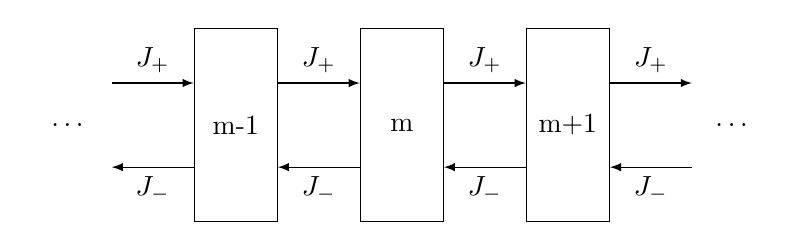
\begin{tikzpicture}[>=latex]
          %[set style={{help lines}+=[dashed]}, scale=0.85, 
          %every node/.style={scale=1}]
          \tikzstyle{state} = [draw, fill=white, rectangle, 
          minimum height=7em, minimum width=3em, node distance=6em]
          \tikzstyle{state2} = [draw=white, fill=white, rectangle, 
          minimum height=7em, minimum width=3em, node distance=6em]
          \tikzstyle{stateEdgePortion} = [black];
          \tikzstyle{stateEdge} = [stateEdgePortion,->];
          \tikzstyle{edgeLabel} = [above, pos=0.5, text centered];
          \tikzstyle{edgeLabel2} = [below, pos=0.5, text centered];
          \node[state] (nodeM) {m-1};
          \node[state, right of=nodeM] (nodeN) {m};
          \node[state, right of=nodeN] (nodeO) {m+1};
          \node[state2, left of=nodeM] (nodeL) {\ldots};
          \node[state2, right of=nodeO] (nodeP) {\ldots};
          
          \draw (nodeM.45)
          edge[stateEdge] node[edgeLabel]{$J_+$} 
          (nodeN.135);
          \draw (nodeN.45)
          edge[stateEdge] node[edgeLabel]{$J_+$} 
          (nodeO.135);
          \draw (nodeO.45)
          edge[stateEdge] node[edgeLabel]{$J_+$} 
          (nodeP.135);
          \draw (nodeL.45)
          edge[stateEdge] node[edgeLabel]{$J_+$} 
          (nodeM.135);
          
          \draw (nodeN.225)
          edge[stateEdge] node[edgeLabel2]{$J_-$} 
          (nodeM.315);
          \draw (nodeP.225)
          edge[stateEdge] node[edgeLabel2]{$J_-$} 
          (nodeO.315);
          \draw (nodeO.225)
          edge[stateEdge] node[edgeLabel2]{$J_-$} 
          (nodeN.315);
          \draw (nodeM.225)
          edge[stateEdge] node[edgeLabel2]{$J_-$} 
          (nodeL.315);
      \end{tikzpicture}
      \begin{block}{Overview}
          \begin{itemize}
              \item Breaks global domain into independent nodes
              \item Nodes are linked by boundary conditions.
              \item Boundary conditions based on truncated, orthogonal 
              basis expansions
              \item Sweep across nodes for global solution
          \end{itemize}
      \end{block}
  \end{frame}
  
%   \begin{frame}
%       \frametitle{Nodal Boundary Conditions}
%       \begin{columns}[c]
%           \begin{column}{0.5\textwidth}
%               \begin{block}{Overview}
%                   \begin{itemize}
%                       \item Break global domain into independent nodes
%                       \item Compute each node individually
%                       \item Recover global solution by sweeping across the nodes
%                   \end{itemize}
%               \end{block}
%           \end{column}
%           \begin{column}{0.5\textwidth}
%               Approximate by Basis Expansion
%               \begin{equation*}
%                   \begin{split}
%                       \psi(g) &= \sum^H_{h=0} a_h P^h(g) \\
%                       a_h &= \sum^G_{g=1} \psi(g) P^h(g)
%                   \end{split}
%               \end{equation*}
%               
%               Codes {\tt Serment} and {\tt Detran} used for calculations
%           \end{column}
%       \end{columns}
%   \end{frame}
  
  \begin{frame}
      \frametitle{Expanding in Energy Groups}
      %     Energy Phase Space discretized by groups
      \begin{columns}[T]
          \begin{column}{0.5\textwidth}
              Approximate by Basis Expansion
              \begin{equation*}
                  \begin{split}
                      \psi(g) &= \sum^H_{h=0} a_h P^h(g) \\
                      a_h &= \sum^G_{g=1} \psi(g) P^h(g)
                  \end{split}
              \end{equation*}
              
              Codes {\tt Serment} and {\tt Detran} used for calculations
          \end{column}
          \begin{column}{0.5\textwidth}
              \begin{block}{Background}
                  \begin{itemize}
                      \item RMM typically uses few (<7) groups
                      \item More groups means greater fidelity
                      \item Fewer DOF mean faster computations
                  \end{itemize}
              \end{block}
          \end{column}
    \end{columns}
  \end{frame}
  
  \begin{frame}
      \frametitle{Why use Response Matrix Methods?}
      \begin{columns}[T]
          \begin{column}{0.5\textwidth}
              \begin{block}{Advantages of RMM}
                  \begin{itemize}
                      \item Quickly reduces the degrees of freedom
                      \item Reduces any/all phase space variables
                      \item Easy to parallelize
                      \item Most effort can be done a priori
                  \end{itemize}
              \end{block}
          \end{column}
          \begin{column}{0.5\textwidth}
              \begin{block}{Disadvantages of RMM}
                  \begin{itemize}
                      \item Computationally Slow
                      \item Limited by Basis Functions
                  \end{itemize}
              \end{block}
              \begin{block}{Number of Responses}
                  Take EO=7, AO=PO=1, SO=2
                  
                  Total responses are
                  
                  $RO = (EO+1)*(SO+1)*$
                  
                  $\quad (PO+1)*(AO+1) = 96$
                  
                  per surface per k per node
                  
              \end{block}
          \end{column}
      \end{columns}
  \end{frame}
  
  \begin{frame}
      \frametitle{Project Goals}
      \begin{block}{Main Objectives}
          \begin{itemize}
              \item Reduce the number of degrees of freedom by an order of 
              magnitude
              \item Resolve pin powers or nodal fission densities to 
              sub-$0.1\%$ relative errors
          \end{itemize}
      \end{block}
      \begin{block}{Approach}
          \begin{itemize}
              \item Determine a successful basis for energy expansion
              \item Determine constituents of an effective KLT basis
          \end{itemize}
      \end{block}
  \end{frame}
  
  \section{Overview of Basis Sets}
  
  \begin{frame}
      \frametitle{The Multigroup Solution and the Kronecker-$\delta$}
      \begin{equation*}
          P_{\delta}^h(g) = \delta_{h, g-1} = 
          \begin{cases}
              1, & \text{if }  h = g-1 \, , \\
              0, & \text{if }  h \neq g-1 \, .
          \end{cases}
          ,\, g=1,\, 2, \, \ldots,\, G \, ,
      \end{equation*}
      \begin{columns}[T]
          \begin{column}{0.5\textwidth}
              For the 4-group case, the Kronecker-$\delta$ vectors are:
              \begin{equation*}
                  \begin{split}
                      &[1,0,0,0] \\
                      &[0,1,0,0] \\
                      &[0,0,1,0] \\
                      &[0,0,0,1]
                  \end{split}
              \end{equation*}
          \end{column}
          \begin{column}{0.5\textwidth}
              \begin{block}{Overview of Kronecker-$\delta$}
                  \begin{itemize}
                      \item Prohibitively expensive with large G
                      \item Cannot truncate the basis set
                      \item Perfect convergence at full order
                  \end{itemize}
              \end{block}
          \end{column}
      \end{columns}
  \end{frame}

  \begin{frame}
      \frametitle{Discrete Legendre Polynomials}
      \begin{columns}[T]
          \begin{column}{0.4\textwidth}
              \begin{block}{Polynomial Basis Set}
                  \begin{itemize}
                      \item Constructed to contain polynomials up to a chosen 
                      order
                      \item An $N$th order polynomial can perfectly fit $N+1$ 
                      points
                  \end{itemize}
              \end{block}
          \end{column}
          \begin{column}{0.6\textwidth}
              \includegraphics[trim=.1cm .25cm .1cm .4cm, clip=true,
              totalheight=0.65\textheight]{Figures/DLP_basis}
          \end{column}
      \end{columns}
  \end{frame}

  \begin{frame}
      \frametitle{Basis Expansion by DLP}
      \centering
      \includegraphics[trim=.1cm .25cm .1cm .4cm, clip=true,
    totalheight=0.65\textheight]{Figures/expansion}
    \begin{block}{}
    Using 40 discrete points, $\cos(x), \, x\in[0,2\pi]$ expanded by 
Discrete Legendre Polynomials to $4^{th}$ order
\end{block}
  \end{frame}

  
  \begin{frame}
      \frametitle{Modified Discrete Legendre Polynomials}
      \begin{columns}[T]
          \begin{column}{0.4\textwidth}
              \begin{block}{Creating mDLPs}
                  \begin{itemize}
                      \item Impose spatially averaged flux profile
                      \item Resulting polynomials are orthogonalized
                      \item Improves DLP by incorporating relevant phase space 
                      information
                  \end{itemize}
              \end{block}
          \end{column}
          \begin{column}{0.6\textwidth}
              \centering
              \only<1>{
                  \includegraphics[trim=.1cm .25cm .1cm .4cm, clip=true,
                  totalheight=0.65\textheight]{Figures/shape}
                  
                  Shape Vector}
              \only<2>{
                  \includegraphics[trim=.1cm .25cm .1cm .4cm, clip=true,
                  totalheight=0.65\textheight]{Figures/mDLP1_L_basis}
                  
                  mDLP Type 1}
              \only<3>{
                  \includegraphics[trim=.1cm .25cm .1cm .4cm, clip=true,
                  totalheight=0.65\textheight]{Figures/mDLP2_L_basis}
                  
                  mDLP Type 2}
          \end{column}
      \end{columns}
  \end{frame}
  
  \begin{frame}
      \frametitle{The Karhunen Lo\'{e}ve Transform}
      \begin{columns}[T]
          \begin{column}{0.5\textwidth}
              \begin{block}{The KLT seeks to}
                  \begin{itemize}
                      \item Construct the most effective basis set
                      \item Capture the problem in a minimal number of basis 
                      functions
                  \end{itemize}
                  
              \end{block}
          \end{column}
          \begin{column}{0.5\textwidth}
              \begin{block}{Applications of KLT}
                  \begin{itemize}
                      \item Image compression
                      \item Reduced-order modeling
                  \end{itemize}
              \end{block}
          \end{column}
      \end{columns}
  \end{frame}

  
  \begin{frame}
      \frametitle{Relating KLT and the SVD}
      \begin{block}{}
          Form matrix $\mathbf{D}$ from snapshots of $\phi$ or other term of 
          interest.
      \end{block}
      \begin{columns}[c]
          \begin{column}{0.5\textwidth}
              \begin{equation*}
              \mathbf{D} = \begin{bmatrix}
                  \phi_{1,1} & \phi_{1,2} & \cdots & \phi_{1,s} \\
                  \phi_{2,1} & \phi_{2,2} & \cdots & \phi_{2,s} \\
                  \vdots & \vdots & \ddots \\
                  \phi_{g,1} & \phi_{g,2} & & \phi_{g,s}
              \end{bmatrix}
          \end{equation*}
          \end{column}
          \begin{column}{0.5\textwidth}
              \begin{equation*}
                  \begin{split}
                      \mathbf{D} &= \mathbf{U} \bm{\Sigma} 
                      \mathbf{V}^{\intercal} \\
                      \mathbf{D}^{\intercal}\mathbf{D}  &= \mathbf{V} 
                      \bm{\Sigma} 
                      \mathbf{U}^{\intercal} \mathbf{U} \bm{\Sigma} 
                      \mathbf{V}^{\intercal} \\
                      &= \mathbf{V} \bm{\Sigma}^2 \mathbf{V}^{\intercal} \\
                      &= \mathbf{Q}\bm{\Lambda}\mathbf{Q}^{\intercal}
                  \end{split}
              \end{equation*}
          \end{column}
      \end{columns}
      \begin{block}{}
          $\mathbf{D}^{\intercal}\mathbf{D}$ is a symmetric positive definite 
          matrix.  Thus, $\mathbf{Q}\bm{\Lambda}\mathbf{Q}^{\intercal}$ exists.
      \end{block}
  \end{frame}

  
  \begin{frame}
      \frametitle{Karhunen Lo\'{e}ve Transform}
      \begin{block}{}
      Form matrix $\mathbf{D}$ from snapshots of $\phi$ or other term of 
      interest.
  \end{block}
      \begin{columns}[c]
          \begin{column}{0.5\textwidth}
              \begin{equation*}
              \mathbf{D} = \begin{bmatrix}
                  \phi_{1,1} & \phi_{1,2} & \cdots & \phi_{1,s} \\
                  \phi_{2,1} & \phi_{2,2} & \cdots & \phi_{2,s} \\
                  \vdots & \vdots & \ddots \\
                  \phi_{g,1} & \phi_{g,2} & & \phi_{g,s}
              \end{bmatrix}
          \end{equation*}
          \end{column}
          \begin{column}{0.5\textwidth}
              \setlength{\mathindent}{0pt}
              \begin{equation*}
                  \begin{split}
                      &\mathbf{B} = \mathbf{D}^{T}\mathbf{D} \\
                      &\mathbf{Bb}_j = \lambda_j \mathbf{b}_j \,  \quad \& \quad 
                      \lambda_j > \lambda_{j+1} \, , \forall j \\
                      &P^j_{KLT}(:) = \mathbf{D}\mathbf{b}_j \\
                      & \mathbf{f} \approx \sum_j a_j P^j_{KLT}(:) \\
                      &a_j 
                      = 
                      \mathbf{f}^T P^j_{KLT}(:)
                  \end{split}
              \end{equation*}
          \end{column}
      \end{columns}
      \begin{block}{}
      After orthogonalization of $P^j_{KLT}(:)$, the KLT generates a 
      number of basis vectors equal to number snapshots (in this case, s).
      \end{block}
  \end{frame}
  
  \begin{frame}
      \frametitle{KLT Basis Vectors}
      \begin{columns}[T]
          \begin{column}{0.4\textwidth}
              \begin{block}{KLT Features}
                  \begin{itemize}
                      \item Problem Specific
                      \item Longer Computation Times
                      \item Highly Efficient
                  \end{itemize}
              \end{block}
          \end{column}
          \begin{column}{0.6\textwidth}
              \includegraphics[trim=.1cm .25cm .1cm .4cm, clip=true,
              totalheight=0.65\textheight]{Figures/KLT_basis}
          \end{column}
      \end{columns}
  \end{frame}
  
  \begin{frame}
      \frametitle{Basis Set Comparison}
      \centering
      \includegraphics[trim=.1cm .25cm .1cm .4cm, clip=true,
      totalheight=0.65\textheight]{Figures/KLT_example}
      \begin{block}{}
          Relative error in the $L_2$ norm as a function of expansion order for 
          KLT compared to other basis sets
      \end{block}

  \end{frame}

  
  \section{Test Problems and Models}
  
  \begin{frame}
      \frametitle{10-pin Test Problem}
      \begin{block}{Pin Cell Mesh}
          \begin{itemize}
              \item 22 mesh cells of fuel 
              \item 3 mesh cells of moderator on either side
              \item Each pin cell provides 28 energy-dependent snapshots
          \end{itemize}
      \end{block}
      \centering
          \begin{figure}
              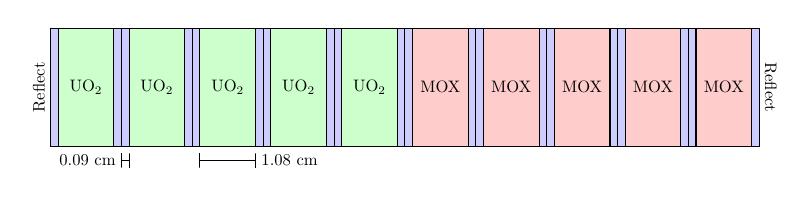
\begin{tikzpicture}[scale=0.6, every node/.style={scale=0.6}]
                  \foreach \x in {0,1.5,...,6}
                  \filldraw[xshift=\x cm, fill=green!20!white, draw=black] 
                  (0.160714286,0) rectangle (1.339285714,2.5) node[pos=.5] 
                  {UO$_2$};
                  \foreach \x in {7.5,9,...,13.5}
                  \filldraw[xshift=\x cm, fill=red!20!white, draw=black] 
                  (0.160714286,0) rectangle (1.339285714,2.5) node[pos=.5] 
                  {MOX};
                  \foreach \x in {0,1.5,...,13.5}
                  \filldraw[xshift=\x cm, fill=blue!20!white, draw=black] (0,0) 
                  rectangle (0.160714286,2.5);
                  \foreach \x in {0,1.5,...,13.5}
                  \filldraw[xshift=\x cm, fill=blue!20!white, draw=black] 
                  (1.339285714,0) rectangle (1.5,2.5);
                  \draw[xshift=15cm,yshift=1.25cm] node[right] 
                  {\rotatebox{-90}{Reflect}};
                  \draw[yshift=1.25cm] node[left] {\rotatebox{90}{Reflect}};
                  \draw (1.5,-.15) -- (1.5,-.45) -- (1.5,-.30) node[left] {0.09 
                      cm} -- (1.660714286,-.30) -- (1.660714286,-.15) -- 
                  (1.660714286, -.45);
                  \draw (3.160714286,-.15) -- (3.160714286,-.45) -- 
                  (3.160714286,-.30) -- (4.339285714,-.30) node[right] {1.08 
cm}                   -- (4.339285714,-.15) -- (4.339285714, -.45);
              \end{tikzpicture}
          \end{figure}
      
      \begin{block}{Test Problem Settings}
          \begin{itemize}
              \item 16-angle, double Gauss-Legendre quadrature
              \item Step characteristic spatial discretization
          \end{itemize}
      \end{block}
  \end{frame}
  
  \begin{frame}
    \frametitle{10-pin Snapshot Models}
    \begin{table}
      \begin{tabular}{l | p{7cm}}\toprule
	Abbreviation    & Model to generate snapshots \\ \midrule
        Full-Assembly   & Repeating array of 10 UO$_2$ and 10 MOX pins \\
        N-pin           & Repeating array of N UO$_2$ and N MOX pins \\ 
        Combined-Pins   & Combined snapshots from UO$_2$ and MOX models, and 
        two-pin, UO$_2$-MOX model \\
        UO$_2$-Pin      & UO$_2$ pin only \\
        MOX-Pin         & MOX pin only \\
        \bottomrule
      \end{tabular}
      \label{tab:snapshots}
    \end{table}
  \end{frame}
  
    \begin{frame}
    \frametitle{BWR Test Problem}
    \centering
    Assemblies and pin cells had reflective conditions.
    
    \begin{figure}
      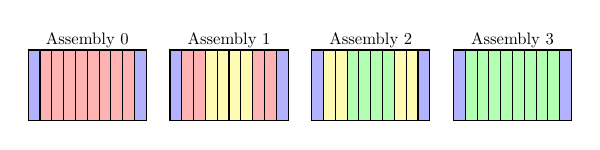
\begin{tikzpicture}[scale=0.6, every node/.style={scale=0.6}]
            \foreach \x in {0,2.25,3,5.25,6,8.25,9,11.25}
            \filldraw[xshift=\x cm,fill=blue!30!white,draw=black] (0,0) 
            rectangle (0.25,1.5);
            \foreach \x in {.25,.5,.75,1,1.25,1.5,1.75,2,3.25,3.5,4.75,5}
            \filldraw[xshift=\x cm,fill=red!30!white,draw=black] (0,0) 
            rectangle (0.25,1.5);
            \foreach \x in {3.75,4,4.25,4.5,6.25,6.5,7.75,8}
            \filldraw[xshift=\x cm,fill=yellow!30!white,draw=black] (0,0) 
            rectangle (0.25,1.5);
            \foreach \x in 
            {6.75,7,7.25,7.5,9.25,9.5,9.75,10,10.25,10.5,10.75,11}
            \filldraw[xshift=\x cm,fill=green!30!white,draw=black] (0,0) 
            rectangle (0.25,1.5);
            \draw (0.25,1.7) node[right] {Assembly 0};%
            \draw (3.25,1.7) node[right] {Assembly 1};%
            \draw (6.25,1.7) node[right] {Assembly 2};%
            \draw (9.25,1.7) node[right] {Assembly 3};%
      \end{tikzpicture}
    \end{figure}
    \begin{figure}
      \vspace*{-.35cm}
      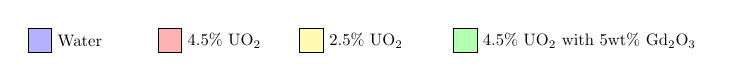
\begin{tikzpicture}[scale=0.6, every node/.style={scale=0.6}]
\filldraw[xshift=-4cm,fill=blue!30!white,draw=black] (-.25,-.25) 
            rectangle (.25,.25) node[yshift=-.25cm, right] {Water};%
            \filldraw[xshift=-1.25cm,fill=red!30!white,draw=black] (-.25,-.25) 
            rectangle (.25,.25) node[yshift=-.25cm, right] {4.5$\%$ UO$_2$};%
            \filldraw[xshift=1.75cm,fill=yellow!30!white,draw=black] 
            (-.25,-.25) rectangle (.25,.25) node[yshift=-.25cm, 
            right] {2.5$\%$ UO$_2$};%
            \filldraw[xshift=5cm,fill=green!30!white,draw=black] (-.25,-.25) 
            rectangle (.25,.25) node[yshift=-.25cm, right] {4.5$\%$ UO$_2$ with 
            5wt$\%$ Gd$_2$O$_3$};%
      \end{tikzpicture}
    \end{figure}
    \begin{figure}
      \vspace*{-.35cm}
      
\begin{tikzpicture}
\foreach \x in {0,.1,...,6.9}
            \filldraw[xshift=\x cm,fill=red!30!white,draw=black] (0,0) 
            rectangle (0.1,.75);
            \foreach \x in {0,1,2,3,4,5,6,.9,1.9,2.9,3.9,4.9,5.9,6.9}
            \filldraw[xshift=\x cm,fill=blue!30!white,draw=black] (0,0) 
            rectangle (0.1,.75);
            \foreach \x in {1.3,1.4,1.5,1.6,3.3,3.4,3.5,3.6,5.3,5.4,5.5,5.6}
            \filldraw[xshift=\x cm,fill=yellow!30!white,draw=black] (0,0) 
            rectangle (0.1,.75);
            \draw (7,.375) node[right] {Core 0};%
            \draw (0,.375) node[left,color=white] {Core 0};
      \end{tikzpicture}
    \end{figure}
    \begin{figure}
      \vspace*{-.35cm}
      
\begin{tikzpicture}
            \foreach \x in {0,.1,...,6.9}
            \filldraw[xshift=\x cm,fill=red!30!white,draw=black] (0,0) 
            rectangle (0.1,.75);
            \foreach \x in {0,1,2,3,4,5,6,.9,1.9,2.9,3.9,4.9,5.9,6.9}
            \filldraw[xshift=\x cm,fill=blue!30!white,draw=black] (0,0) 
            rectangle (0.1,.75);
            \foreach \x in {1.1,1.2,1.7,1.8,3.1,3.2,3.7,3.8,5.1,5.2,5.7,5.8}
            \filldraw[xshift=\x cm,fill=yellow!30!white,draw=black] (0,0) 
            rectangle (0.1,.75);
            \foreach \x in {1.3,1.4,1.5,1.6,3.3,3.4,3.5,3.6,5.3,5.4,5.5,5.6}
            \filldraw[xshift=\x cm,fill=green!30!white,draw=black] (0,0) 
            rectangle (0.1,.75);
            \draw (7,.375) node[right] {Core 1};%
            \draw (0,.375) node[left,color=white] {Core 1};
      \end{tikzpicture}
    \end{figure}
    \begin{figure}
      \vspace*{-.35cm}
      
\begin{tikzpicture}
            \foreach \x in {0,.1,...,6.9}
            \filldraw[xshift=\x cm,fill=red!30!white,draw=black] (0,0) 
            rectangle (0.1,.75);
            \foreach \x in {0,1,2,3,4,5,6,.9,1.9,2.9,3.9,4.9,5.9,6.9}
            \filldraw[xshift=\x cm,fill=blue!30!white,draw=black] (0,0) 
            rectangle (0.1,.75);
            \foreach \x in {1.1,1.2,1.3,1.4,1.5,1.6,1.7,1.8, 
                            3.1,3.2,3.3,3.4,3.5,3.6,3.7,3.8,
                            5.1,5.2,5.3,5.4,5.5,5.6,5.7,5.8}
            \filldraw[xshift=\x cm,fill=green!30!white,draw=black] (0,0) 
            rectangle (0.1,.75);
            \draw (7,.375) node[right] {Core 2};%
            \draw (0,.375) node[left,color=white] {Core 2};
      \end{tikzpicture}
    \end{figure}
    Core models had vacuum boundary conditions.
    
  \end{frame}
  
  \begin{frame}
      \frametitle{BWR Test Problem}
      \begin{columns}[T]
          \begin{column}{0.5\textwidth}
              \begin{block}{Pin Cell Mesh}
                  \begin{itemize}
                      \item 16 mesh cells of fuel 
                      \item 6 mesh cells of moderator on either side
                      \item Each pin cell provides 28 energy-dependent snapshots
                  \end{itemize}
              \end{block}
          \end{column}
          \begin{column}{0.5\textwidth}
              \centering
              \begin{figure}
                  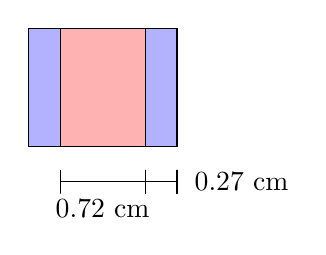
\begin{tikzpicture}[scale=1.5, every node/.style={scale=1}]
                      \filldraw[xshift=0 cm, yshift=0 cm, fill=blue!30!white, 
                      draw=black] 
                      (0, 0) rectangle (1.26,1.0) node[pos=.5] {};
                      \filldraw[xshift=0 cm, yshift=0 cm, fill=red!30!white, 
                      draw=black] 
                      (0.27,0) rectangle (0.99,1.0) node[pos=.5] {};
                      \draw (.27,-.2) -- (.27,-.4) -- (.27,-.30) -- (0.63,-.3) 
                      node[below=0.1cm] 
                      {0.72 cm} -- (.99,-.30) -- (.99,-.2) -- (.99, -.4);
                      \draw (.99,-.2) -- (.99,-.4) -- (.99,-.30) --  (1.26,-.30)
                      node[right=0.1cm] 
                      {0.27 cm} -- (1.26,-.30) -- (1.26,-.2) -- (1.26, -.4);
                  \end{tikzpicture}
              \end{figure}
          \end{column}
      \end{columns}
      \begin{block}{Test Problem Settings}
          \begin{itemize}
              \item 16-angle, double Gauss-Legendre quadrature
              \item Step characteristic spatial discretization
          \end{itemize}
      \end{block}
  \end{frame}
 
  
  \begin{frame}
    \frametitle{BWR Snapshot Models}
    \begin{table}
      \begin{tabular}{l | p{6cm}}\toprule
        Abbreviation         & Model to generate snapshots \\ \midrule
        Full-Core            & Snapshots from whole core model (i.e., the test 
        problem) \\
        Combined-Assemblies  & Snapshots from unique assemblies used in core 
        configuration \\
        Combined-Pins        & Snapshots from unique pins used in core 
        configuration \\
        \bottomrule
      \end{tabular}
      \label{tab:bwrsnapshots}
    \end{table}
  \end{frame}
 
  \begin{frame}
      \frametitle{C5G7 Test Problem}
      \begin{columns}[T]
          \begin{column}{0.5\textwidth}
      \begin{block}{Pin Cell Mesh}
          \begin{itemize}
              \item 7$\times$7 Cartesian mesh
              \item Each pin cell provides 49 energy-dependent snapshots
          \end{itemize}
      \end{block}
  \end{column}
  \begin{column}{0.5\textwidth}
      \centering
          \begin{figure}
              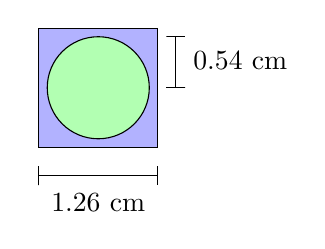
\begin{tikzpicture}[scale=1.2, every node/.style={scale=1}]
        \filldraw[xshift=0 cm, yshift=0 cm, fill=blue!30!white, draw=black] 
        (0, 0) rectangle (1.26,1.26) node[pos=.5] {};
        \filldraw[xshift=0 cm, yshift=0 cm, fill=green!30!white, draw=black] 
        (.63,.63) circle (.54) node[pos=.5] {};
        \draw (0,-.2) -- (0,-.4) -- (0,-.30) -- (0.63,-.3) node[below=0.1cm] 
        {1.26 cm} -- (1.26,-.30) -- (1.26,-.2) -- (1.26, -.4);
        \draw (1.35,.63) -- (1.55,.63) -- (1.45,.63) -- (1.45,.92) 
        node[right=0.1cm] {0.54 cm} -- (1.45,1.17) -- (1.35,1.17) -- (1.55, 
        1.17);
    \end{tikzpicture}
          \end{figure}
  \end{column}
\end{columns}
      \begin{block}{Test Problem Settings}
          \begin{itemize}
              \item 16-angle, Gauss-Chebyshev quadrature for polar angle
              \item 16-angle, Abu-Shumays Quadruple Range quadrature for 
azimuthal angle
              \item Diamond difference spatial discretization
              \item Scale-generated, 44-group Cross-section Library
          \end{itemize}
      \end{block}
      
  \end{frame}
  
  \begin{frame}
      \frametitle{C5G7 Core Configuration}
      \begin{figure}
          \only<1>{
    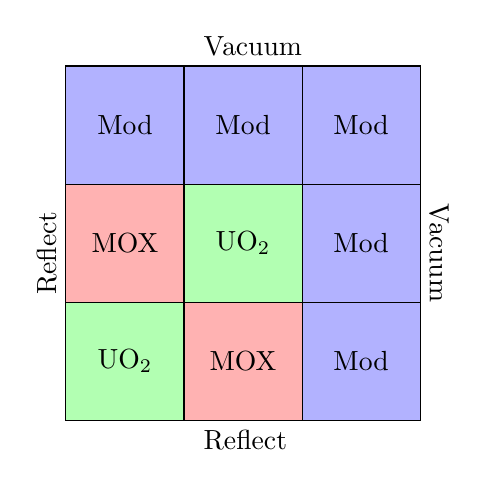
\begin{tikzpicture}[scale=0.5, every node/.style={scale=1}]
        \filldraw[xshift=6 cm, yshift=0 cm, fill=blue!30!white, draw=black] 
        (0, 0) rectangle (3,3) node[pos=.5] {Mod};
        \filldraw[xshift=6 cm, yshift=3 cm, fill=blue!30!white, draw=black] 
        (0, 0) rectangle (3,3) node[pos=.5] {Mod};
        \filldraw[xshift=6 cm, yshift=6 cm, fill=blue!30!white, draw=black] 
        (0, 0) rectangle (3,3) node[pos=.5] {Mod};
        \filldraw[xshift=3 cm, yshift=6 cm, fill=blue!30!white, draw=black] 
        (0, 0) rectangle (3,3) node[pos=.5] {Mod};
        \filldraw[xshift=0 cm, yshift=6 cm, fill=blue!30!white, draw=black] 
        (0, 0) rectangle (3,3) node[pos=.5] {Mod};
        \filldraw[xshift=0 cm, yshift=0 cm, fill=green!30!white, draw=black] 
        (0, 0) rectangle (3,3) node[pos=.5] {UO$_2$};
        \filldraw[xshift=3 cm, yshift=3 cm, fill=green!30!white, draw=black] 
        (0, 0) rectangle (3,3) node[pos=.5] {UO$_2$};
        \filldraw[xshift=3 cm, yshift=0 cm, fill=red!30!white, draw=black] 
        (0, 0) rectangle (3,3) node[pos=.5] {MOX};
        \filldraw[xshift=0 cm, yshift=3 cm, fill=red!30!white, draw=black] 
        (0, 0) rectangle (3,3) node[pos=.5] {MOX};
        \draw[xshift=9cm,yshift=4.25cm] node[right] 
        {\rotatebox{-90}{Vacuum}};
        \draw[yshift=4.25cm] node[left] {\rotatebox{90}{Reflect}};
        \draw[xshift=3.25cm,yshift=9.5cm] node[right] {{Vacuum}};
        \draw[xshift=3.25cm, yshift=-.5cm] node[right] {{Reflect}};
    \end{tikzpicture}}
\only<2>{
    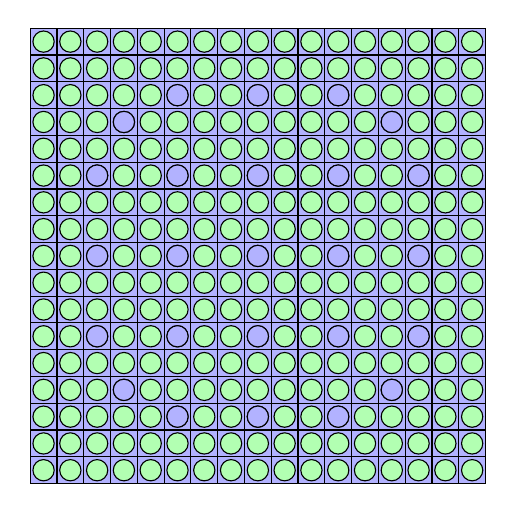
\begin{tikzpicture}[scale=0.27, every node/.style={scale=1}]
        \foreach \x in {0,1.26,...,20.16}
        \foreach \y in {0,1.26,...,20.16}
        \filldraw[xshift=\x cm, yshift=\y cm, fill=blue!30!white, 
        draw=black] (0, 0) rectangle (1.26,1.26) node[pos=.5] {};
        \foreach \x in {0,1.26,...,20.16}
        \foreach \y in {0,1.26,...,20.16}
        \filldraw[xshift=\x cm, yshift=\y cm, fill=green!30!white, 
        draw=black] (.63,.63) circle (.5) node[pos=.5] {};
        \foreach \x in {5*1.26, 8*1.26, 11*1.26}
        \foreach \y in {2*1.26, 14*1.26}
        \filldraw[xshift=\x cm, yshift=\y cm, fill=blue!30!white, 
        draw=black] (.63,.63) circle (.5) node[pos=.5] {};
        \foreach \x in {3*1.26, 13*1.26}
        \foreach \y in {3*1.26, 13*1.26}
        \filldraw[xshift=\x cm, yshift=\y cm, fill=blue!30!white, 
        draw=black] (.63,.63) circle (.5) node[pos=.5] {};
        \foreach \x in {2*1.26, 5*1.26, 8*1.26, 11*1.26, 14*1.26}
        \foreach \y in {5*1.26, 8*1.26, 11*1.26}
        \filldraw[xshift=\x cm, yshift=\y cm, fill=blue!30!white, 
        draw=black] (.63,.63) circle (.5) node[pos=.5] {};
    \end{tikzpicture}}
\only<3>{
    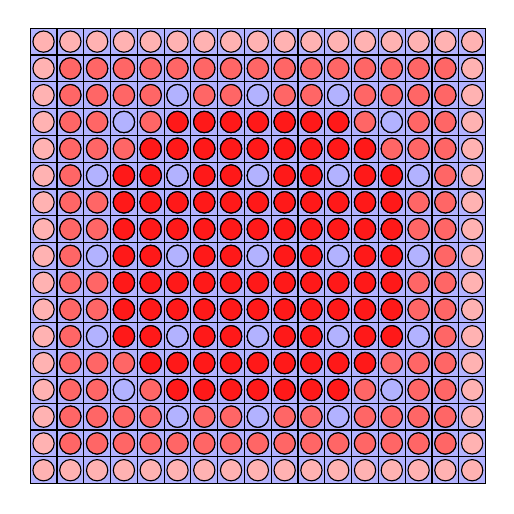
\begin{tikzpicture}[scale=0.27, every node/.style={scale=1}]
        \foreach \x in {0,1.26,...,20.16}
        \foreach \y in {0,1.26,...,20.16}
        \filldraw[xshift=\x cm, yshift=\y cm, fill=blue!30!white, 
        draw=black] (0, 0) rectangle (1.26,1.26) node[pos=.5] {};
        \foreach \x in {0,1.26,...,20.16}
        \foreach \y in {0,1.26,...,20.16}
        \filldraw[xshift=\x cm, yshift=\y cm, fill=red!30!white, draw=black] 
        (.63,.63) circle (.5) node[pos=.5] {};
        \foreach \x in {1.26,2.52,...,20.16}
        \foreach \y in {1.26,2.52,...,20.16}
        \filldraw[xshift=\x cm, yshift=\y cm, fill=red!60!white, draw=black] 
        (.63,.63) circle (.5) node[pos=.5] {};
        \foreach \x in {5*1.26,6*1.26,7*1.26,8*1.26,9*1.26,10*1.26,11*1.26}
        \foreach \y in {3*1.26,13*1.26}
        \filldraw[xshift=\x cm, yshift=\y cm, fill=red!90!white, draw=black] 
        (.63,.63) circle (.5) node[pos=.5] {};
        \foreach \x in 
        {4*1.26,5*1.26,6*1.26,7*1.26,8*1.26,9*1.26,10*1.26,11*1.26,12*1.26}
        \foreach \y in {4*1.26,12*1.26}
        \filldraw[xshift=\x cm, yshift=\y cm, fill=red!90!white, draw=black] 
        (.63,.63) circle (.5) node[pos=.5] {};
        \foreach \x in {3.78,5.04,...,16.38}
        \foreach \y in {6.3,7.56,...,15.04}
        \filldraw[xshift=\x cm, yshift=\y cm, fill=red!90!white, draw=black] 
        (.63,.63) circle (.5) node[pos=.5] {};
        \foreach \x in {5*1.26, 8*1.26, 11*1.26}
        \foreach \y in {2*1.26, 14*1.26}
        \filldraw[xshift=\x cm, yshift=\y cm, fill=blue!30!white, 
        draw=black] (.63,.63) circle (.5) node[pos=.5] {};
        \foreach \x in {3*1.26, 13*1.26}
        \foreach \y in {3*1.26, 13*1.26}
        \filldraw[xshift=\x cm, yshift=\y cm, fill=blue!30!white, 
        draw=black] (.63,.63) circle (.5) node[pos=.5] {};
        \foreach \x in {2*1.26, 5*1.26, 8*1.26, 11*1.26, 14*1.26}
        \foreach \y in {5*1.26, 8*1.26, 11*1.26}
        \filldraw[xshift=\x cm, yshift=\y cm, fill=blue!30!white, 
        draw=black] (.63,.63) circle (.5) node[pos=.5] {};
    \end{tikzpicture}}
\end{figure}  
    \begin{figure}
        \centering
      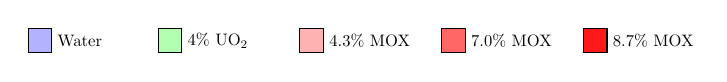
\begin{tikzpicture}[scale=0.6, every node/.style={scale=0.6}]
\filldraw[xshift=-4cm,fill=blue!30!white,draw=black] (-.25,-.25) 
            rectangle (.25,.25) node[yshift=-.25cm, right] {Water};%
            \filldraw[xshift=-1.25cm,fill=green!30!white,draw=black] 
(-.25,-.25) 
            rectangle (.25,.25) node[yshift=-.25cm, right] {4$\%$ UO$_2$};%
            \filldraw[xshift=1.75cm,fill=red!30!white,draw=black] 
            (-.25,-.25) rectangle (.25,.25) node[yshift=-.25cm, 
            right] {4.3$\%$ MOX};%
            \filldraw[xshift=4.75cm,fill=red!60!white,draw=black] 
            (-.25,-.25) rectangle (.25,.25) node[yshift=-.25cm, 
            right] {7.0$\%$ MOX};%
            \filldraw[xshift=7.75cm,fill=red!90!white,draw=black] 
            (-.25,-.25) rectangle (.25,.25) node[yshift=-.25cm, 
            right] {8.7$\%$ MOX};%
      \end{tikzpicture}
    \end{figure}
\end{frame}

\begin{frame}
    \frametitle{C5G7 Snapshot Models}
    \begin{table}
        \resizebox{0.9\columnwidth}{!}{%
            \begin{tabular}{l | p{8cm}}\toprule
                Abbreviation         & Model to generate snapshots \\ \midrule
                Reduced Full-Core    & Spatially averaged snapshots from whole 
                core 
                model (i.e.,         the test problem) \\
                Combined-Assemblies  & Snapshots from assemblies used in core 
                configuration \\
                Combined-Pins        & Snapshots from pins used in core 
                configuration combined with the pin 
                junctions\\
                Small-Core           & Snapshots from the small core model \\
                Small-Assemblies     & Snapshots from the small assemblies used 
                in the 
                small core configuration \\
                Reduced Small-Core   & Spatially averaged snapshots from the 
                small core 
                model \\
                1-D Approximation    & Snapshots from the 1-D approximation to 
                the C5G7 
                benchmark \\
        \bottomrule
    \end{tabular}}
    \end{table}
  \end{frame}
  
  \begin{frame}
      \frametitle{Snapshot Model Configurations}
      \only<1>{
          \begin{block}{}
              \centering
              Pincell Junction Configuration
          \end{block}
          
          \begin{figure}
              \centering
              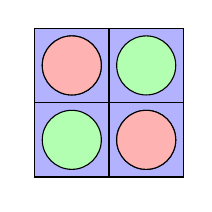
\begin{tikzpicture}[scale=0.75, every node/.style={scale=1}]
                  \foreach \x in {0,1.26}
                  \foreach \y in {0,1.26}
                  \filldraw[xshift=\x cm, yshift=\y cm, fill=blue!30!white, 
                  draw=black] (0, 0) rectangle (1.26,1.26) node[pos=.5] {};
                  \foreach \x in {0,1.26}
                  \foreach \y in {0,1.26}
                  \filldraw[xshift=\x cm, yshift=\y cm, fill=green!30!white, 
                  draw=black] (.63,.63) circle (.5) node[pos=.5] {};
                  \filldraw[xshift=0 cm, yshift=1.26 cm, fill=red!30!white, 
                  draw=black] (.63,.63) circle (.5) node[pos=.5] {};
                  \filldraw[xshift=1.26 cm, yshift=0 cm, fill=red!30!white, 
                  draw=black] (.63,.63) circle (.5) node[pos=.5] {};
              \end{tikzpicture}
          \end{figure}}
      \only<2>{
          \begin{block}{}
              \centering
              Small Core Configuration
          \end{block}
          \begin{columns}[T]
              \begin{column}{0.5\textwidth}
                  \begin{figure}
                      \centering
                      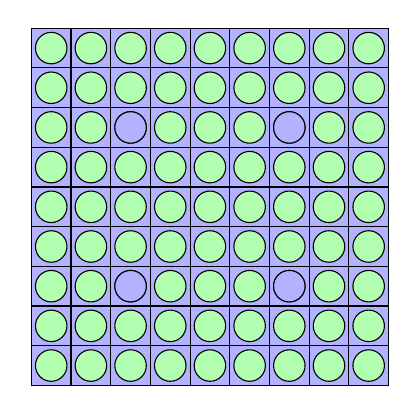
\begin{tikzpicture}[scale=0.4, every 
                          node/.style={scale=1}]
                          \foreach \x in {0,1.26,...,10.08}
                          \foreach \y in {0,1.26,...,10.08}
                          \filldraw[xshift=\x cm, yshift=\y cm, 
                          fill=blue!30!white, 
                          draw=black] (0, 0) rectangle (1.26,1.26) node[pos=.5] 
                          {};
                          \foreach \x in {0,1.26,...,10.08}
                          \foreach \y in {0,1.26,...,10.08}
                          \filldraw[xshift=\x cm, yshift=\y cm, 
                          fill=green!30!white, 
                          draw=black] (.63,.63) circle (.5) node[pos=.5] {};
                          \foreach \x in {2*1.26, 6*1.26}
                          \foreach \y in {2*1.26, 6*1.26}
                          \filldraw[xshift=\x cm, yshift=\y cm, 
                          fill=blue!30!white, 
                          draw=black] (.63,.63) circle (.5) node[pos=.5] {};
                      \end{tikzpicture}
                  \end{figure}
              \end{column}
              \begin{column}{0.5\textwidth}
                  \begin{figure}
                      \centering
                      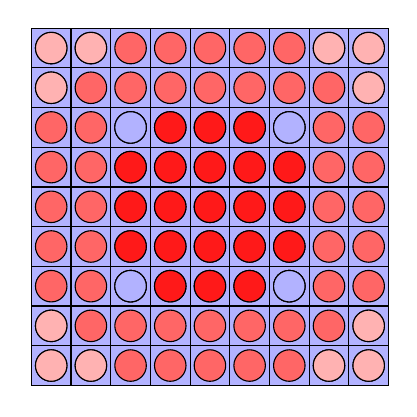
\begin{tikzpicture}[scale=0.4, every 
                          node/.style={scale=1}]
                          \foreach \x in {0,1.26,...,10.08}
                          \foreach \y in {0,1.26,...,10.08}
                          \filldraw[xshift=\x cm, yshift=\y cm, 
                          fill=blue!30!white, 
                          draw=black] (0, 0) rectangle (1.26,1.26) node[pos=.5] 
                          {};
                          \foreach \x in {0,1.26,...,10.08}
                          \foreach \y in {0,1.26,...,10.08}
                          \filldraw[xshift=\x cm, yshift=\y cm, 
                          fill=red!60!white,                       draw=black] 
                          (.63,.63) circle (.5) node[pos=.5] {};
                          \foreach \x in {0,1.26,7*1.26,10.08}
                          \foreach \y in {0,10.08}
                          \filldraw[xshift=\x cm, yshift=\y cm, 
                          fill=red!30!white,                       draw=black] 
                          (.63,.63) circle (.5) node[pos=.5] {};
                          \foreach \x in {0,10.08}
                          \foreach \y in {1.26,7*1.26}
                          \filldraw[xshift=\x cm, yshift=\y cm, 
                          fill=red!30!white,                       draw=black] 
                          (.63,.63) circle (.5) node[pos=.5] {};
                          \foreach \x in {2.52,3.78,...,7.56}
                          \foreach \y in {2.52,3.78,...,7.56}
                          \filldraw[xshift=\x cm, yshift=\y cm, 
                          fill=red!90!white,                       draw=black] 
                          (.63,.63) circle (.5) node[pos=.5] {};
                          \foreach \x in {2*1.26, 6*1.26}
                          \foreach \y in {2*1.26, 6*1.26}
                          \filldraw[xshift=\x cm, yshift=\y cm, 
                          fill=blue!30!white, 
                          draw=black] (.63,.63) circle (.5) node[pos=.5] {};
                  \end{tikzpicture}
                  \end{figure}
              \end{column}
          \end{columns}}
      \only<3>{
          \begin{block}{}
              \centering
              1-D Approximation Configuration
          \end{block}
          \begin{figure}
        \centering
        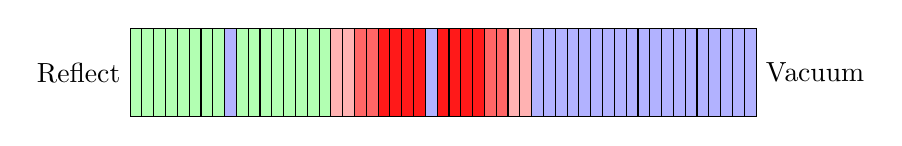
\begin{tikzpicture}[scale=1.5, every node/.style={scale=1}]
            \foreach \x in {0,.1,...,1.7}
            \filldraw[xshift=\x cm,fill=green!30!white,draw=black] (0,0) 
            rectangle (0.1,.75);
            \foreach \x in {1.7,1.8,...,3.4}
            \filldraw[xshift=\x cm,fill=red!30!white,draw=black] (0,0) 
            rectangle (0.1,.75);
            \foreach \x in {1.9,2.0,...,3.2}
            \filldraw[xshift=\x cm,fill=red!60!white,draw=black] (0,0) 
            rectangle (0.1,.75);
            \foreach \x in {2.1,2.2,...,2.9}
            \filldraw[xshift=\x cm,fill=red!90!white,draw=black] (0,0) 
            rectangle (0.1,.75);
            \foreach \x in {3.4,3.5,...,5.3}
            \filldraw[xshift=\x cm,fill=blue!30!white,draw=black] (0,0) 
            rectangle (0.1,.75);
            \foreach \x in {0.8,2.5}
            \filldraw[xshift=\x cm,fill=blue!30!white,draw=black] (0,0) 
            rectangle (0.1,.75);
            \draw (5.3,.375) node[right] {Vacuum};%
            \draw (0,.375) node[left] {Reflect};
        \end{tikzpicture}
    \end{figure}
    \begin{figure}
        \centering
        \vspace*{-0.65 cm}
        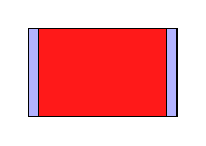
\begin{tikzpicture}[scale=1.5, every node/.style={scale=1}]
            \filldraw[xshift=0 cm,fill=blue!30!white,draw=black] (0,0) 
            rectangle (.09,.75);
            \filldraw[xshift=.09 cm,fill=red!90!white,draw=black] (0,0) 
            rectangle (1.17,.75);
            \filldraw[xshift=1.17 cm,fill=blue!30!white,draw=black] (0,0) 
            rectangle (.09,.75);
        \end{tikzpicture}
    \end{figure}}
    \begin{figure}
        \centering
      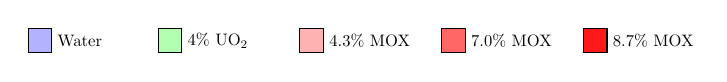
\begin{tikzpicture}[scale=0.6, every node/.style={scale=0.6}]
\filldraw[xshift=-4cm,fill=blue!30!white,draw=black] (-.25,-.25) 
            rectangle (.25,.25) node[yshift=-.25cm, right] {Water};%
            \filldraw[xshift=-1.25cm,fill=green!30!white,draw=black] 
(-.25,-.25) 
            rectangle (.25,.25) node[yshift=-.25cm, right] {4$\%$ UO$_2$};%
            \filldraw[xshift=1.75cm,fill=red!30!white,draw=black] 
            (-.25,-.25) rectangle (.25,.25) node[yshift=-.25cm, 
            right] {4.3$\%$ MOX};%
            \filldraw[xshift=4.75cm,fill=red!60!white,draw=black] 
            (-.25,-.25) rectangle (.25,.25) node[yshift=-.25cm, 
            right] {7.0$\%$ MOX};%
            \filldraw[xshift=7.75cm,fill=red!90!white,draw=black] 
            (-.25,-.25) rectangle (.25,.25) node[yshift=-.25cm, 
            right] {8.7$\%$ MOX};%
      \end{tikzpicture}
    \end{figure}
      \end{frame}
      
      \begin{frame}
          \frametitle{Work Flowchart}
          \centering
          \begin{figure}
\tikzstyle{process} = [rectangle, rounded corners, minimum width=3cm, minimum 
height=1cm,text centered, draw=black, fill=structure!30!white]
\tikzstyle{arrow} = [thick,->,>=stealth]
\scalebox{0.8}{
\begin{tikzpicture}[node distance=1.3cm]
    \node (snapshots) [process] {Generate Snapshots with {\tt Detran}};
    \node (reference) [process, below of=snapshots] {Generate Multigroup 
        Reference Solution with {\tt Serment}};
    \node (KLT) [process, below of=reference] {Generate Basis Functions};
    \node (Databases) [process, below of=KLT] {Generate Response Databases for 
        each case};
    \node (Process) [process, below of=Databases] {Solve Test Problem using 
        Database with {\tt Serment}};
        \node (Error) [process, below of=Process] {Compare Solution to 
Reference};
    \draw [arrow] (snapshots) -- (reference);
    \draw [arrow] (reference) -- (KLT);
    \draw [arrow] (KLT) -- (Databases);
    \draw [arrow] (Databases) -- (Process);
    \draw [arrow] (Process) -- (Error);
\end{tikzpicture}}
\end{figure}
      \end{frame}

  \begin{frame}
      \frametitle{Project Goals}
      \begin{block}{Main Objectives}
          \begin{itemize}
              \item Reduce the number of degrees of freedom by an order of 
              magnitude
              \item Resolve pin powers or nodal fission densities to 
              sub-$0.1\%$ relative errors
          \end{itemize}
      \end{block}
      \begin{block}{Approach}
          \begin{itemize}
              \item Determine a successful basis for energy expansion
              \item Determine constituents of an effective KLT basis
          \end{itemize}
      \end{block}
  \end{frame}
  
  \section{Results and Analysis}
  
  \begin{frame}
      \frametitle{Types of Results}
      \begin{block}{Snapshot Types}
          \begin{itemize}
              \item Scalar Flux $\phi$
              \item Partial Current $J_-$
              \item Higher-Order Angular Moments
          \end{itemize}

      \end{block}
      \begin{block}{Combinations of Snapshots}
          \begin{itemize}
              \item Only $\phi$
              \item Only $J_-$
              \item Combined $\phi$ and $J_-$
              \item Only Higher-Order Moments
              \item Combined $\phi$, $J_-$, and Higher Moments
          \end{itemize}

      \end{block}

  \end{frame}

  \begin{frame}
      \frametitle{Results of DLP and mDLP}
      \centering
      Comparison of DLP and mDLP for 10-pin problem
      \begin{figure}
          \includegraphics[trim=.1cm .25cm 2.0cm .4cm clip=true,%
          totalheight=0.75\textheight]{Figures/c/10-pin/44/rf_plots/phi/%
              mDLP_comparison_fission-44}
      \end{figure}
  \end{frame}
  
  \begin{frame}
    \frametitle{10-pin 44-group Library}
    \centering
    Using snapshots of only $\phi$
    \begin{figure}
    \includegraphics[trim=.1cm .25cm 2.0cm .4cm clip=true, 
    totalheight=0.75\textheight]{Figures/c/10-pin/44/rf_plots/phi/%
        energy_basis_comparison_fission-44}
    \end{figure}
  \end{frame}
  
  \begin{frame}
    \frametitle{10-pin 44-group Library}
    \centering
    Using snapshots of only $J_-$
    \begin{figure}
    \includegraphics[trim=.1cm .25cm 2.0cm .4cm clip=true, 
    totalheight=0.75\textheight]{Figures/s/10-pin/44/rf_plots/partial/%
        partial_energy_basis_comparison_fission-44}
    \end{figure}
  \end{frame}
  
  \begin{frame}
    \frametitle{10-pin 44-group Library}
    \centering
    Using snapshots of $\phi$ and $J_-$
    \begin{figure}
    \includegraphics[trim=.1cm .25cm 2.0cm .4cm clip=true, 
    totalheight=0.75\textheight]{Figures/c/10-pin/44/rf_plots/partial/%
        partial_energy_basis_comparison_fission-44}
    \end{figure}
  \end{frame}
  
  \begin{frame}
    \frametitle{10-pin 44-group Library}
    \centering
    Using snapshots of only Higher-Order Angular Moments for Full-Assembly 
model.
    \begin{figure}
    \includegraphics[trim=.1cm .25cm 2.0cm .4cm clip=true, 
    totalheight=0.75\textheight]{Figures/s/10-pin/44/rf_plots/angular/%
        angular_comparison_fission_10-pin-44}
    \end{figure}
  \end{frame}
  
  \begin{frame}
    \frametitle{10-pin 44-group Library}
    \centering
    Using snapshots of $\phi$, $J_-$, and Higher-Order Angular Moments  for 
Full-Assembly 
model.
    \begin{figure}
    \includegraphics[trim=.1cm .25cm 2.0cm .4cm clip=true, 
    totalheight=0.75\textheight]{Figures/c/10-pin/44/rf_plots/angular/%
        angular_comparison_fission_10-pin-44}
    \end{figure}
  \end{frame}
  
  \begin{frame}
      \frametitle{10-pin 238-group Library}
      \centering
      Using snapshots of only $\phi$
      \begin{figure}
        \begin{columns}[T]
            \begin{column}{0.5\textwidth}
                \resizebox{\textwidth}{!}{
                \includegraphics[trim=.1cm .25cm 2.0cm .4cm clip=true, 
                ]{Figures/c/10-pin/238/rf_plots/phi/%
                    energy_basis_comparison_fission-44}}
          \end{column}
        \begin{column}{0.5\textwidth}
            \resizebox{\textwidth}{!}{
              \includegraphics[trim=.1cm .25cm 2.0cm .4cm clip=true, 
              ]{Figures/c/10-pin/238/rf_plots/phi/%
                  energy_basis_comparison_fission-238}}
          \end{column}
      \end{columns}
  \end{figure}
  \end{frame}
  
    \begin{frame}
      \frametitle{10-pin 238-group Library}
      \centering
      Using snapshots of only $J_-$
      \begin{figure}
        \begin{columns}[T]
            \begin{column}{0.5\textwidth}
                \resizebox{\textwidth}{!}{
                \includegraphics[trim=.1cm .25cm 2.0cm .4cm clip=true, 
                ]{Figures/s/10-pin/238/rf_plots/partial/%
            partial_energy_basis_comparison_fission-44}}
          \end{column}
        \begin{column}{0.5\textwidth}
            \resizebox{\textwidth}{!}{
              \includegraphics[trim=.1cm .25cm 2.0cm .4cm clip=true, 
              ]{Figures/s/10-pin/238/rf_plots/partial/%
            partial_energy_basis_comparison_fission-238}}
          \end{column}
      \end{columns}
  \end{figure}
  \end{frame}
 
  \begin{frame}
      \frametitle{10-pin 238-group Library}
      \centering
      Using snapshots of $\phi$ and $J_-$
      \begin{figure}
          \begin{columns}[T]
              \begin{column}{0.5\textwidth}
                  \resizebox{\textwidth}{!}{
                      \includegraphics[trim=.1cm .25cm 2.0cm .4cm clip=true, 
                      ]{Figures/c/10-pin/238/rf_plots/partial/%
                          partial_energy_basis_comparison_fission-44}}
              \end{column}
              \begin{column}{0.5\textwidth}
                  \resizebox{\textwidth}{!}{
                      \includegraphics[trim=.1cm .25cm 2.0cm .4cm clip=true, 
                      ]{Figures/c/10-pin/238/rf_plots/partial/%
                          partial_energy_basis_comparison_fission-238}}
              \end{column}
          \end{columns}
      \end{figure}
  \end{frame}
  
%   \begin{frame}
%       \frametitle{10-pin 238-group Library}
%       \centering
%       Using snapshots of only Higher-Order Angular Moments for Full-Assembly 
% model.
%       \begin{figure}
%           \begin{columns}[T]
%               \begin{column}{0.5\textwidth}
%                   \resizebox{\textwidth}{!}{
%                       \includegraphics[trim=.1cm .25cm 2.0cm .4cm clip=true, 
%                       ]{Figures/s/10-pin/238/rf_plots/angular/%
%             angular_comparison_fission_10-pin-44}}
%               \end{column}
%               \begin{column}{0.5\textwidth}
%                   \resizebox{\textwidth}{!}{
%                       \includegraphics[trim=.1cm .25cm 2.0cm .4cm clip=true, 
%                       ]{Figures/s/10-pin/238/rf_plots/angular/%
%             angular_comparison_fission_10-pin-238}}
%               \end{column}
%           \end{columns}
%       \end{figure}
%   \end{frame}
%   
%     \begin{frame}
%       \frametitle{10-pin 238-group Library}
%       \centering
%       Using snapshots of $\phi$, $J_-$, and Higher-Order Angular Moments for 
% Full-Assembly 
% model.
%       \begin{figure}
%           \begin{columns}[T]
%               \begin{column}{0.5\textwidth}
%                   \resizebox{\textwidth}{!}{
%                       \includegraphics[trim=.1cm .25cm 2.0cm .4cm clip=true, 
%                       ]{Figures/c/10-pin/238/rf_plots/angular/%
%             angular_comparison_fission_10-pin-44}}
%               \end{column}
%               \begin{column}{0.5\textwidth}
%                   \resizebox{\textwidth}{!}{
%                       \includegraphics[trim=.1cm .25cm 2.0cm .4cm clip=true, 
%                       ]{Figures/c/10-pin/238/rf_plots/angular/%
%             angular_comparison_fission_10-pin-238}}
%               \end{column}
%           \end{columns}
%       \end{figure}
%   \end{frame}
  
  \begin{frame}
    \frametitle{BWR Core-0 44-group Library}
    \centering
    Using snapshots of only $\phi$
    \begin{figure}
    \includegraphics[trim=.1cm .25cm 2.0cm .4cm clip=true, 
    totalheight=0.75\textheight]{Figures/c/bwrcore/44/0/rf_plots/phi/%
        energy_basis_comparison_fission-44}
    \end{figure}
  \end{frame}
  
  \begin{frame}
    \frametitle{BWR Core-0 44-group Library}
    \centering
    Using snapshots of only $J_-$
    \begin{figure}
    \includegraphics[trim=.1cm .25cm 2.0cm .4cm clip=true, 
    totalheight=0.75\textheight]{Figures/s/bwrcore/44/0/rf_plots/partial/%
        partial_energy_basis_comparison_fission-44}
    \end{figure}
  \end{frame}
  
  \begin{frame}
    \frametitle{BWR Core-0 44-group Library}
    \centering
    Using snapshots of $\phi$ and $J_-$
    \begin{figure}
    \includegraphics[trim=.1cm .25cm 2.0cm .4cm clip=true, 
    totalheight=0.75\textheight]{Figures/c/bwrcore/44/0/rf_plots/partial/%
        partial_energy_basis_comparison_fission-44}
    \end{figure}
  \end{frame}
  
    \begin{frame}
      \frametitle{BWR Core-0 238-group Library}
      \centering
      Using snapshots of only $\phi$
      \begin{figure}
        \begin{columns}[T]
            \begin{column}{0.5\textwidth}
                \resizebox{\textwidth}{!}{
                \includegraphics[trim=.1cm .25cm 2.0cm .4cm clip=true, 
                ]{Figures/c/bwrcore/238/0/rf_plots/phi/%
        energy_basis_comparison_fission-44}}
          \end{column}
        \begin{column}{0.5\textwidth}
            \resizebox{\textwidth}{!}{
              \includegraphics[trim=.1cm .25cm 2.0cm .4cm clip=true, 
              ]{Figures/c/bwrcore/238/0/rf_plots/phi/%
        energy_basis_comparison_fission-238}}
          \end{column}
      \end{columns}
  \end{figure}
  \end{frame}
  
    \begin{frame}
      \frametitle{BWR Core-0 238-group Library}
      \centering
      Using snapshots of only $J_-$
      \begin{figure}
        \begin{columns}[T]
            \begin{column}{0.5\textwidth}
                \resizebox{\textwidth}{!}{
                \includegraphics[trim=.1cm .25cm 2.0cm .4cm clip=true, 
                ]{Figures/s/bwrcore/238/0/rf_plots/partial/%
        partial_energy_basis_comparison_fission-44}}
          \end{column}
        \begin{column}{0.5\textwidth}
            \resizebox{\textwidth}{!}{
              \includegraphics[trim=.1cm .25cm 2.0cm .4cm clip=true, 
              ]{Figures/s/bwrcore/238/0/rf_plots/partial/%
        partial_energy_basis_comparison_fission-238}}
          \end{column}
      \end{columns}
  \end{figure}
  \end{frame}
 
  \begin{frame}
      \frametitle{BWR Core-0 238-group Library}
      \centering
      Using snapshots of $\phi$ and $J_-$
      \begin{figure}
          \begin{columns}[T]
              \begin{column}{0.5\textwidth}
                  \resizebox{\textwidth}{!}{
                      \includegraphics[trim=.1cm .25cm 2.0cm .4cm clip=true, 
                      ]{Figures/c/bwrcore/238/0/rf_plots/partial/%
        partial_energy_basis_comparison_fission-44}}
              \end{column}
              \begin{column}{0.5\textwidth}
                  \resizebox{\textwidth}{!}{
                      \includegraphics[trim=.1cm .25cm 2.0cm .4cm clip=true, 
                      ]{Figures/c/bwrcore/238/0/rf_plots/partial/%
        partial_energy_basis_comparison_fission-238}}
              \end{column}
          \end{columns}
      \end{figure}
  \end{frame}
  
  \begin{frame}
    \frametitle{BWR Core-2 44-group Library}
    \centering
    Using snapshots of only $\phi$
    \begin{figure}
    \includegraphics[trim=.1cm .25cm 2.0cm .4cm clip=true, 
    totalheight=0.75\textheight]{Figures/c/bwrcore/44/2/rf_plots/phi/%
        energy_basis_comparison_fission-44}
    \end{figure}
  \end{frame}
  
  \begin{frame}
    \frametitle{BWR Core-2 44-group Library}
    \centering
    Using snapshots of only $J_-$
    \begin{figure}
    \includegraphics[trim=.1cm .25cm 2.0cm .4cm clip=true, 
    totalheight=0.75\textheight]{Figures/s/bwrcore/44/2/rf_plots/partial/%
        partial_energy_basis_comparison_fission-44}
    \end{figure}
  \end{frame}
  
  \begin{frame}
    \frametitle{BWR Core-2 44-group Library}
    \centering
    Using snapshots of $\phi$ and $J_-$
    \begin{figure}
    \includegraphics[trim=.1cm .25cm 2.0cm .4cm clip=true, 
    totalheight=0.75\textheight]{Figures/c/bwrcore/44/2/rf_plots/partial/%
        partial_energy_basis_comparison_fission-44}
    \end{figure}
  \end{frame}
  
    \begin{frame}
      \frametitle{BWR Core-2 238-group Library}
      \centering
      Using snapshots of only $\phi$
      \begin{figure}
        \begin{columns}[T]
            \begin{column}{0.5\textwidth}
                \resizebox{\textwidth}{!}{
                \includegraphics[trim=.1cm .25cm 2.0cm .4cm clip=true, 
                ]{Figures/c/bwrcore/238/2/rf_plots/phi/%
        energy_basis_comparison_fission-44}}
          \end{column}
        \begin{column}{0.5\textwidth}
            \resizebox{\textwidth}{!}{
              \includegraphics[trim=.1cm .25cm 2.0cm .4cm clip=true, 
              ]{Figures/c/bwrcore/238/2/rf_plots/phi/%
        energy_basis_comparison_fission-238}}
          \end{column}
      \end{columns}
  \end{figure}
  \end{frame}
  
    \begin{frame}
      \frametitle{BWR Core-2 238-group Library}
      \centering
      Using snapshots of only $J_-$
      \begin{figure}
        \begin{columns}[T]
            \begin{column}{0.5\textwidth}
                \resizebox{\textwidth}{!}{
                \includegraphics[trim=.1cm .25cm 2.0cm .4cm clip=true, 
                ]{Figures/s/bwrcore/238/2/rf_plots/partial/%
        partial_energy_basis_comparison_fission-44}}
          \end{column}
        \begin{column}{0.5\textwidth}
            \resizebox{\textwidth}{!}{
              \includegraphics[trim=.1cm .25cm 2.0cm .4cm clip=true, 
              ]{Figures/s/bwrcore/238/2/rf_plots/partial/%
        partial_energy_basis_comparison_fission-238}}
          \end{column}
      \end{columns}
  \end{figure}
  \end{frame}
 
  \begin{frame}
      \frametitle{BWR Core-2 238-group Library}
      \centering
      Using snapshots of $\phi$ and $J_-$
      \begin{figure}
          \begin{columns}[T]
              \begin{column}{0.5\textwidth}
                  \resizebox{\textwidth}{!}{
                      \includegraphics[trim=.1cm .25cm 2.0cm .4cm clip=true, 
                      ]{Figures/c/bwrcore/238/2/rf_plots/partial/%
        partial_energy_basis_comparison_fission-44}}
              \end{column}
              \begin{column}{0.5\textwidth}
                  \resizebox{\textwidth}{!}{
                      \includegraphics[trim=.1cm .25cm 2.0cm .4cm clip=true, 
                      ]{Figures/c/bwrcore/238/2/rf_plots/partial/%
        partial_energy_basis_comparison_fission-238}}
              \end{column}
          \end{columns}
      \end{figure}
  \end{frame}
  
    \begin{frame}
    \frametitle{C5G7 44-group Library - Nodal Fission Density Results}
    \centering
    Using snapshots of only $\phi$
    \begin{figure}
    \includegraphics[trim=.1cm .25cm 2.0cm .4cm clip=true, 
    totalheight=0.75\textheight]{Figures/c/c5g7/rf_plots/phi/%
        energy_basis_comparison_fission-10}
    \end{figure}
  \end{frame}
  
  \begin{frame}
    \frametitle{C5G7 44-group Library - Nodal Fission Density Results}
    \centering
    Using snapshots of $\phi$, $J_{up}$, and $J_{down}$
    \begin{figure}
    \includegraphics[trim=.1cm .25cm 2.0cm .4cm clip=true, 
    totalheight=0.75\textheight]{Figures/c/c5g7/rf_plots/partial/%
        partial_energy_basis_comparison_fission-10}
    \end{figure}
  \end{frame}
  
   \begin{frame}
    \frametitle{C5G7 44-group Library - Pin Power Results}
    \centering
    Using snapshots of only $\phi$
    \begin{figure}
    \includegraphics[trim=.1cm .25cm 2.0cm .4cm clip=true, 
    totalheight=0.75\textheight]{Figures/c/c5g7/rf_plots/phi/%
        energy_basis_comparison_pinpower-10}
    \end{figure}
  \end{frame}
  
  \begin{frame}
    \frametitle{C5G7 44-group Library - Pin Power Results}
    \centering
    Using snapshots of $\phi$, $J_{up}$, and $J_{down}$
    \begin{figure}
    \includegraphics[trim=.1cm .25cm 2.0cm .4cm clip=true, 
    totalheight=0.75\textheight]{Figures/c/c5g7/rf_plots/partial/%
        partial_energy_basis_comparison_pinpower-10}
    \end{figure}
  \end{frame}
  
  \begin{frame}
      \frametitle{C5G7 44-group Library - Pin Power Heat Map}
      \centering
      Pin power heat map for the {\tt Detran} reference solution.  The 
      upper left corner is the center of the core
      \begin{figure}
          \includegraphics[trim=.1cm .25cm 2.0cm .4cm clip=true, 
          totalheight=0.75\textheight]{Figures/c/c5g7/rf_plots/%
              c5g7_ref_detran}
      \end{figure}
  \end{frame}
  
  \begin{frame}
      \frametitle{C5G7 44-group Library - Pin Power Heat Map}
      \centering
      Error of pin powers in the {\tt Serment} reference 
      solution relative to the {\tt Detran} reference solution.
      \begin{columns}[T]
          \begin{column}{0.5\textwidth}
              \begin{figure}
                  \resizebox{\textwidth}{!}{
                      \includegraphics[trim=.1cm .25cm 2.0cm .4cm clip=true, 
                      totalheight=0.75\textheight]{Figures/c/c5g7/rf_plots/%
                          detser_error}}
              \end{figure}
          \end{column}
          \begin{column}{0.5\textwidth}
              \begin{block}{Statistics}
                  \begin{itemize}
                      \item Max: 11.09 \%
                      \item Min: 0.0038 \%
                      \item Ave: 1.89 \%
                      \item St. Dev: 1.677 \%
                  \end{itemize}
              \end{block}
          \end{column}
      \end{columns}
  \end{frame}
  
  \begin{frame}
      \frametitle{C5G7 44-group Library - Pin Power Heat Map}
      \centering
      Error in the pin powers of 9th order, Reduced Small-Core, snapshots of 
      $\phi$ case relative to {\tt Serment} 
      reference.  
      \begin{columns}[T]
          \begin{column}{0.5\textwidth}
              \begin{figure}
                  \resizebox{\textwidth}{!}{
                      \includegraphics[trim=.1cm .25cm 2.0cm .4cm clip=true, 
                      totalheight=0.75\textheight]{Figures/c/c5g7/rf_plots/%
                          phi/serklt8_error}}
              \end{figure}
          \end{column}
          \begin{column}{0.5\textwidth}
              \begin{figure}
                  \resizebox{\textwidth}{!}{
                      \includegraphics[trim=.1cm .25cm 2.0cm .4cm clip=true, 
                      totalheight=0.75\textheight]{Figures/c/c5g7/rf_plots/%
                          error1}}
              \end{figure}
          \end{column}
      \end{columns}
  \end{frame}
  
  \begin{frame}
      \frametitle{C5G7 44-group Library - Pin Power Heat Map}
      \centering
      Error in the pin powers of 9th order, Reduced Small-Core, snapshots of 
$\phi$, $J_{up}$, and $J_{down}$ case relative to the 
      {\tt Serment} reference solution.
      \begin{columns}[T]
          \begin{column}{0.5\textwidth}
              \begin{figure}
                  \resizebox{\textwidth}{!}{
                      \includegraphics[trim=.1cm .25cm 2.0cm .4cm clip=true, 
                      totalheight=0.75\textheight]{Figures/c/c5g7/rf_plots/%
                          partial/partial_serklt8_error}}
              \end{figure}
          \end{column}
          \begin{column}{0.5\textwidth}
              \begin{figure}
                  \resizebox{\textwidth}{!}{
                      \includegraphics[trim=.1cm .25cm 2.0cm .4cm clip=true, 
                      totalheight=0.75\textheight]{Figures/c/c5g7/rf_plots/%
                          partial_error1}}
              \end{figure}
          \end{column}
      \end{columns}
  \end{frame}
  
  \section{Concluding Remarks}
  
  \begin{frame}
      \frametitle{Test Problem Conclusions}
      \begin{block}{10-pin Test Problem Conclusions}
          \begin{itemize}
              \item KLT can make highly successful basis sets
              \item Snapshots similar to the test problem improve the results
              \item Additional snapshots only improve results if distinct
              \item Surprisingly, higher-order moments do not lead to better 
              basis functions
              \item Successful KLT functions use all material types
          \end{itemize}
      \end{block}
  \end{frame}
  
  \begin{frame}
      \frametitle{Test Problem Conclusions}
      \begin{block}{BWR Test Problem Conclusions}
          \begin{itemize}
              \item Success of KLT is problem dependent
              \item More difficult problems require more basis functions
          \end{itemize}
      \end{block}
      \begin{block}{C5G7 Test Problem Conclusions}
          \begin{itemize}
              \item Material junctions are hardest to capture
              \item Spatially averaging snapshots provides similar results
          \end{itemize}
      \end{block}
  \end{frame}
  
  
  \begin{frame}
    \frametitle{Concluding Remarks}
    \begin{block}{The Karhunen Lo\'{e}ve Transform :}
      \begin{itemize}
	\item Shows improvement over mDLP
	\item Reduces DOF needed for accurate results
	\item Generally improves with increased information
	\item Can achieves sub $0.1\%$ error with $<1/10$ DOF for some cases
    \item Practical snapshot models provide encouraging results
      \end{itemize}
    \end{block}
\end{frame}

\begin{frame}
    \frametitle{Future Work}
    \begin{block}{Future Work}
      \begin{itemize}
	\item Further explore 2-D problems
    \begin{itemize}
        \item Higher spatial and angular expansion orders
        \item Higher Energy order
    \end{itemize}
	\item More energy group structures
	\item Greater snapshot variety (e.g., angular variation)
    \item Use KLT basis sets to expand {\tt Serment} solution directly
    \item Application of KLT to additional phase-space expansions
      \end{itemize}
    \end{block}
    %\begin{block}{Contact Information}
    %  \begin{itemize}
%	\item Richard Reed: blkpawn@k-state.edu
%	\item Dr. Jeremy Roberts: jaroberts@k-state.edu
%      \end{itemize}
%    \end{block}
    \nocite{*}
  \end{frame}
  
  \begin{frame}
      \frametitle{Acknowledgements}
      \begin{block}{}
              Prof. Jeremy Roberts
              
              Prof. Ken Shultis
              
              Prof. Hitesh Bendra
              
              Prof. Larry Erickson
              
              Lyric, Kevin, and Richard
              
              NRC and the KSU Nuclear Research Fellowship Program
      \end{block}
      Thank you for your attention!
  \end{frame}

  
  \begin{frame}[t,allowframebreaks]\label{lastframe}
    \frametitle{References}
    \bibliographystyle{ans}
    {\scriptsize \bibliography{bibliography}}
  \end{frame}
  
  \beginbackup
  
    \begin{frame}[noframenumbering]
    \frametitle{BWR Core-1 44-group Library}
    \centering
    Using snapshots of only $\phi$
    \begin{figure}
    \includegraphics[trim=.1cm .25cm 2.0cm .4cm clip=true, 
    totalheight=0.75\textheight]{Figures/c/bwrcore/44/1/rf_plots/phi/%
        energy_basis_comparison_fission-44}
    \end{figure}
  \end{frame}
  
  \begin{frame}[noframenumbering]
    \frametitle{BWR Core-1 44-group Library}
    \centering
    Using snapshots of only $J_-$
    \begin{figure}
    \includegraphics[trim=.1cm .25cm 2.0cm .4cm clip=true, 
    totalheight=0.75\textheight]{Figures/s/bwrcore/44/1/rf_plots/partial/%
        partial_energy_basis_comparison_fission-44}
    \end{figure}
  \end{frame}
  
  \begin{frame}[noframenumbering]
    \frametitle{BWR Core-1 44-group Library}
    \centering
    Using snapshots of $\phi$ and $J_-$
    \begin{figure}
    \includegraphics[trim=.1cm .25cm 2.0cm .4cm clip=true, 
    totalheight=0.75\textheight]{Figures/c/bwrcore/44/1/rf_plots/partial/%
        partial_energy_basis_comparison_fission-44}
    \end{figure}
  \end{frame}
  
    \begin{frame}[noframenumbering]
      \frametitle{BWR Core-1 238-group Library}
      \centering
      Using snapshots of only $\phi$
      \begin{figure}
        \begin{columns}[T]
            \begin{column}{0.5\textwidth}
                \resizebox{\textwidth}{!}{
                \includegraphics[trim=.1cm .25cm 2.0cm .4cm clip=true, 
                ]{Figures/c/bwrcore/238/1/rf_plots/phi/%
        energy_basis_comparison_fission-44}}
          \end{column}
        \begin{column}{0.5\textwidth}
            \resizebox{\textwidth}{!}{
              \includegraphics[trim=.1cm .25cm 2.0cm .4cm clip=true, 
              ]{Figures/c/bwrcore/238/1/rf_plots/phi/%
        energy_basis_comparison_fission-238}}
          \end{column}
      \end{columns}
  \end{figure}
  \end{frame}
  
    \begin{frame}[noframenumbering]
      \frametitle{BWR Core-1 238-group Library}
      \centering
      Using snapshots of only $J_-$
      \begin{figure}
        \begin{columns}[T]
            \begin{column}{0.5\textwidth}
                \resizebox{\textwidth}{!}{
                \includegraphics[trim=.1cm .25cm 2.0cm .4cm clip=true, 
                ]{Figures/s/bwrcore/238/1/rf_plots/partial/%
        partial_energy_basis_comparison_fission-44}}
          \end{column}
        \begin{column}{0.5\textwidth}
            \resizebox{\textwidth}{!}{
              \includegraphics[trim=.1cm .25cm 2.0cm .4cm clip=true, 
              ]{Figures/s/bwrcore/238/1/rf_plots/partial/%
        partial_energy_basis_comparison_fission-238}}
          \end{column}
      \end{columns}
  \end{figure}
  \end{frame}
 
  \begin{frame}[noframenumbering]
      \frametitle{BWR Core-1 238-group Library}
      \centering
      Using snapshots of $\phi$ and $J_-$
      \begin{figure}
          \begin{columns}[T]
              \begin{column}{0.5\textwidth}
                  \resizebox{\textwidth}{!}{
                      \includegraphics[trim=.1cm .25cm 2.0cm .4cm clip=true, 
                      ]{Figures/c/bwrcore/238/1/rf_plots/partial/%
        partial_energy_basis_comparison_fission-44}}
              \end{column}
              \begin{column}{0.5\textwidth}
                  \resizebox{\textwidth}{!}{
                      \includegraphics[trim=.1cm .25cm 2.0cm .4cm clip=true, 
                      ]{Figures/c/bwrcore/238/1/rf_plots/partial/%
        partial_energy_basis_comparison_fission-238}}
              \end{column}
          \end{columns}
      \end{figure}
  \end{frame}
  
  \begin{frame}[noframenumbering]
      \frametitle{Energy Spectra for 10-pin Test Problem}
      \centering
      \begin{figure}
          \begin{columns}[T]
              \begin{column}{0.5\textwidth}
                  \resizebox{\textwidth}{!}{
                      \includegraphics[trim=.1cm .25cm 2.0cm .4cm clip=true, 
                      ]{Figures/c/10-pin/44/reference_figures/%
                          44group_spectra_energy}}
                  
                  \centering
                  44-group library
              \end{column}
              \begin{column}{0.5\textwidth}
                  \resizebox{\textwidth}{!}{
                      \includegraphics[trim=.1cm .25cm 2.0cm .4cm clip=true, 
                      ]{Figures/c/10-pin/238/reference_figures/%
                          238group_spectra_energy}}
                 
                  \centering
                  238-group library
              \end{column}
          \end{columns}
      \end{figure}
  \end{frame}
  
    \begin{frame}[noframenumbering]
      \frametitle{Energy Spectra for BWR Test Problem with 44-group 
          library}
      \centering
      \begin{figure}
          \begin{columns}[T]
              \begin{column}{0.5\textwidth}
                  \resizebox{\textwidth}{!}{
                      \includegraphics[trim=.1cm .25cm 2.0cm .4cm clip=true, 
                      ]{Figures/c/bwrcore/44/0/reference_figures/%
                          44group_spectra_energy}}
                  
                  \centering                  
                  Core-0
              \end{column}
              \begin{column}{0.5\textwidth}
                  \resizebox{\textwidth}{!}{
                      \includegraphics[trim=.1cm .25cm 2.0cm .4cm clip=true, 
                      ]{Figures/c/bwrcore/44/2/reference_figures/%
                          44group_spectra_energy}}
                  
                  \centering                  
                  Core-2
              \end{column}
          \end{columns}
      \end{figure}
  \end{frame}
  
  \begin{frame}[noframenumbering]
      \frametitle{Energy Spectra for BWR Test Problem with 238-group 
          library}
      \centering
      \begin{figure}
          \begin{columns}[T]
              \begin{column}{0.5\textwidth}
                  \resizebox{\textwidth}{!}{
                      \includegraphics[trim=.1cm .25cm 2.0cm .4cm clip=true, 
                      ]{Figures/c/bwrcore/238/0/reference_figures/%
                          238group_spectra_energy}}
                  
                  \centering                  
                  Core-0
              \end{column}
              \begin{column}{0.5\textwidth}
                  \resizebox{\textwidth}{!}{
                      \includegraphics[trim=.1cm .25cm 2.0cm .4cm clip=true, 
                      ]{Figures/c/bwrcore/238/2/reference_figures/%
                          238group_spectra_energy}}
                  
                  \centering                  
                  Core-2
              \end{column}
          \end{columns}
      \end{figure}
  \end{frame}
  
    \begin{frame}[noframenumbering]
      \frametitle{Energy Spectra for C5G7 Test Problem}
      \centering
      \begin{figure}
          \begin{columns}[T]
              \begin{column}{0.5\textwidth}
                  \resizebox{\textwidth}{!}{
                      \includegraphics[trim=.1cm .25cm 2.0cm .4cm clip=true, 
                      ]{Figures/c/c5g7/reference_figures/%
                          44group_spectra}}
              \end{column}
          \end{columns}
      \end{figure}
  \end{frame}
  
  \begin{frame}[noframenumbering]
      \frametitle{Parametric Study on Snapshot Selection}
      \centering
      Test Problem: 238-group BWR Core-0 Full-Core Model
      \begin{figure}
          \begin{columns}[T]
              \begin{column}{0.5\linewidth}
                  \resizebox{\textwidth}{!}{
                      \includegraphics[trim=.1cm 1.0cm 1.7cm .4cm clip=true, 
                      totalheight=0.23\textheight]{Figures/parametric/%
                          snapcase0_energy_basis_comparison_fission}}
                  Using evenly spaced snapshots
              \end{column}
              \begin{column}{0.5\linewidth}
                  \resizebox{\textwidth}{!}{
                      \includegraphics[trim=.1cm 1.0cm 1.7cm .4cm clip=true, 
                      totalheight=0.23\textheight]{Figures/parametric/%
                          snapcase1_energy_basis_comparison_fission}}
                  Using randomly selected snapshots
              \end{column}
          \end{columns}
      \end{figure}
  \end{frame}
        
  \begin{frame}[noframenumbering]
      \frametitle{Parametric Study on Snapshot Selection}
      \centering
      Test Problem: 238-group BWR Core-0 Full-Core Model
      \begin{figure}
          \begin{columns}[T]
              \begin{column}{0.5\linewidth}
                  \resizebox{\textwidth}{!}{
                      \includegraphics[trim=.1cm 1.0cm 1.7cm .4cm clip=true, 
                      totalheight=0.23\textheight]{Figures/parametric/%
                          snapcase2_energy_basis_comparison_fission}}
                  Using beginning snapshots
              \end{column}
              \begin{column}{0.5\linewidth}
                  \resizebox{\textwidth}{!}{
                      \includegraphics[trim=.1cm 1.0cm 1.7cm .4cm clip=true, 
                      totalheight=0.23\textheight]{Figures/parametric/%
                          snapcase3_energy_basis_comparison_fission}}
                  Using middle snapshots
              \end{column}
          \end{columns}
      \end{figure}
  \end{frame}
  
    \begin{frame}[noframenumbering]
      \frametitle{Parametric Study on Fineness of Mesh}
      \centering
      Test Problem: 44-group 10-pin Full-Assembly Model
      \begin{figure}
                  \resizebox{!}{0.7\textheight}{
                      \includegraphics[trim=.1cm 1.0cm 1.7cm .4cm clip=true, 
                      totalheight=0.23\textheight]{Figures/parametric/%
        number_basis_comparison_fission}}
                  
      \end{figure}
      \centering
      Legend is the total available snapshots
  \end{frame}
  
    \begin{frame}[noframenumbering]
      \frametitle{Parametric Study on Database Parameters}
      \centering
      Test Problem: 238-group BWR Core-0 Full-Core Model
      \begin{figure}
          \begin{columns}[T]
              \begin{column}{0.5\linewidth}
                  \resizebox{\textwidth}{!}{
                      \includegraphics[trim=.1cm 1.0cm 1.7cm .4cm clip=true, 
                      totalheight=0.23\textheight]{Figures/parametric/%
        nK_energy_basis_comparison_fission}}
                  Sensitivity to Number of k Values
              \end{column}
              \begin{column}{0.5\linewidth}
                  \resizebox{\textwidth}{!}{
                      \includegraphics[trim=.1cm 1.0cm 1.7cm .4cm clip=true, 
                      totalheight=0.23\textheight]{Figures/parametric/%
        kdel_energy_basis_comparison_fission}}
                  Sensitivity to $\delta$k size
              \end{column}
          \end{columns}
      \end{figure}
  \end{frame}
  
  \backupend
  
\end{document}
